{\bf Executive summary: the filesystem notion limits our ability to scale processing and has long since been dropped by industry. Astronomy needs to move on.}
\section{Introduction} \label{sec:intro}

Object Stores are nothing new to Astronomy.  \gls{FITS} and \gls{IRAF} tapes are examples
of object stores that were used when file systems were unable to handle the volumes
of data being produced. Even then, standards for migrating from \gls{Object} Store to file
systems were created, allowing for objects to be retrieved into a predefined namespace
on disk.  The explosion of individual \gls{POSIX} disk capacity and \gls{POSIX}-like file systems
have produced generations of researchers who have never used an \gls{Object} Store. While
this growth has supported data systems up till now, the size and complexity of
data being produced by surveys and even pointed telescope archives is reaching
scales where the requirements placed on file access by the \gls{POSIX} standard are
significantly hindering our ability to work with data.  Different parallel file systems
have different strengths and weaknesses.

At large scale, data service providers such as Dropbox and \gls{AWS} do not store files
in \gls{POSIX} systems.  Rather they present the illusion of directory structure layered over
large scale object stores. This allows for faster file access, with only \gls{CRUD} style
functions taking place on each object.  Further, as the pseudo-filesystem layer is simply a
view of structure typically provided by a graph database, users can arrange or potentially
have real time query driven structure for the file organization, removing how many now
organize data through a sea of nested symlinks.
Some provide local \gls{POSIX} caches of that users view of the
pseudo-filesystem, allowing for \gls{POSIX} style applications to access the files with
fopen, fscan, and fclose standard commands. Additionally, these providers do
not show users how data are stored. One can simply request data in the format
needed (e.g. Excel, \gls{CSV}, or as I assume it is the \gls{JSON} format the web apps
use for sheets).   At scale, applications often forgo
such Posix layers and simply use the \gls{CRUD} interfaces to the objects to load them into
memory, act on the objects, and then update or delete them, in the format they need
as input and with the format they naively produce. Further, the data providers need
not update their data archive when formats change, simply provide a new updated
data access format that can be fueled by legacy data formats.

It is time for Astronomy data researchers to follow this curve. As users have migrated
from using tools on their laptops to support collaboration while reducing
individuals need to manage their systems (Jupyter Hubs, Overleaf, Google Slides),
so should astronomical data processing and analysis. We propose the adoption of
a common Astronomical data access \gls{API} layer.


\section{Recommendations }
\begin{enumerate}
 \item Develop a community wide architecture supporting Science as a Service following
	an industry  standard layered architecture for astronomy processing and data access as
depicted in \figref{fig:ci}.


\begin{figure}
\centering
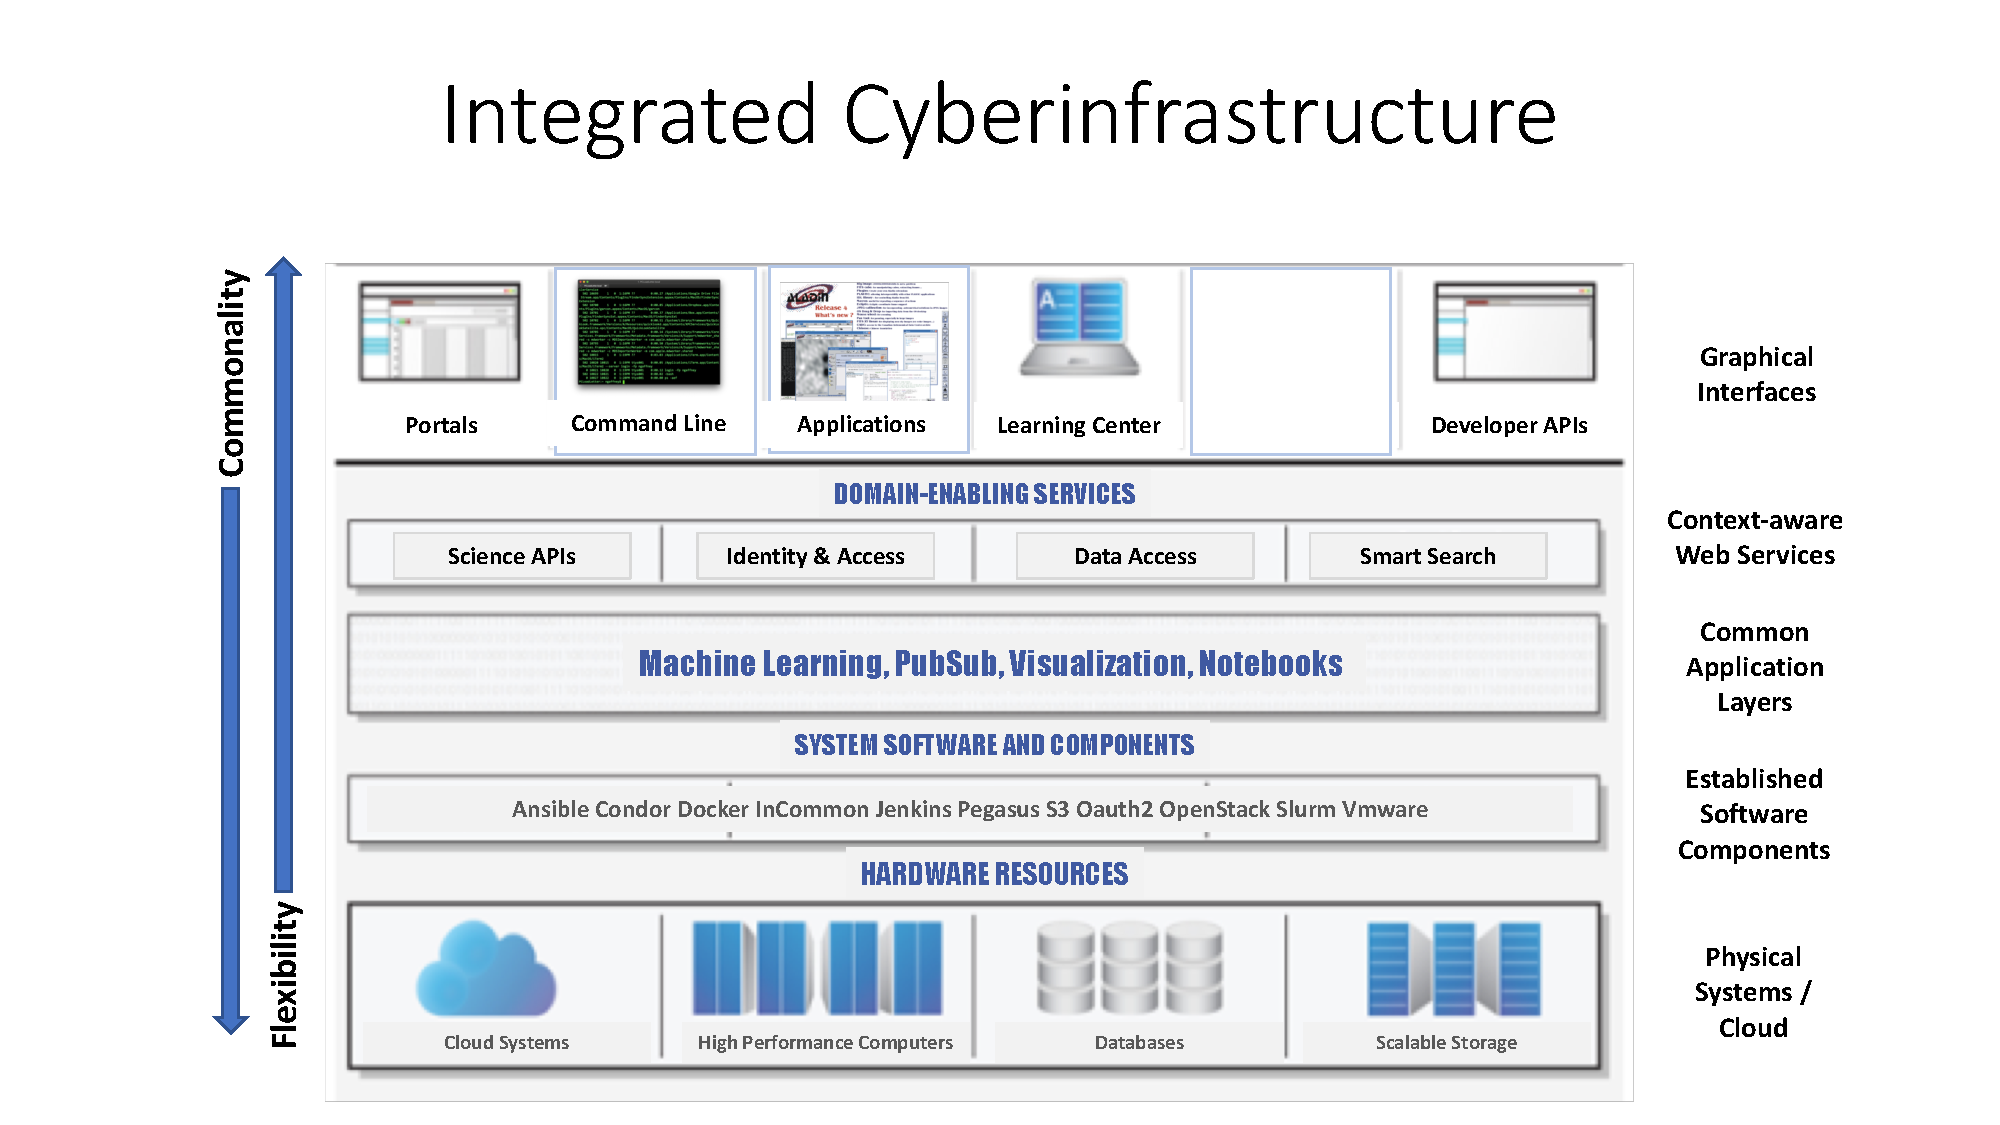
\includegraphics[width=0.49\textwidth]{CI-Layers}
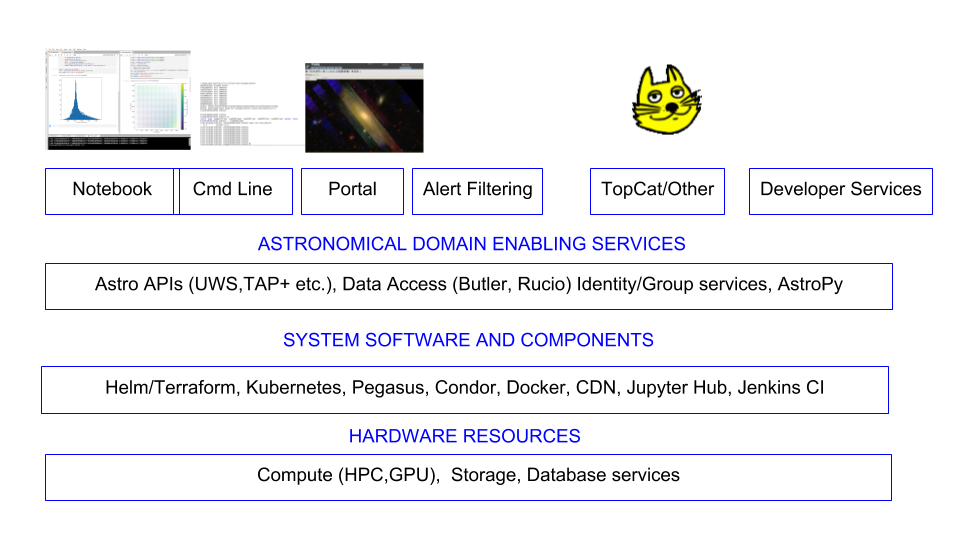
\includegraphics[width=0.49\textwidth]{CI-LSST}
\caption{Industry standard Cyber infrastructure model (left) and an astronomy instantiation of such a model (right)\label{fig:ci}}
\end{figure}

\item Compel all funded funded astronomical projects with \emph{software deliverables} to  leverage the architecture and  APIs for data access.

\item Develop \emph{data and \gls{metadata} transform services}
to support these common \gls{API} layers to aid interoperation.

\item Adopt and subscribe to a \emph{common federated identity service} (e.g. InCommon or
Globus Auth) that is supported by most university and research organizations.
\end{enumerate}




\section{Commodity services and software based community architecture} \label{sec:refarc}
The astronomy and astrophysics community community have historically relied on the development and use of bespoke software and hardware infrastructure to solve challenges related to the managing and analyzing datasets at a scale that was difficult to find in industry or other scientific domains.
These requirements are no longer unique and we have access to a wealth of open source software, commodity hardware, and managed cloud services (offered by commercial providers and federally-funded institutions) that are well positioned to meet the needs of astronomers and astrophysicists \cite{2019AAS...23345706M, 2019AAS...23324505B}.
By providing documentation and reference implementations of the “astronomy stack” using these technologies and making it easier for researchers and missions to access cloud computing services, we can reduce operations costs, accelerate time to science, and increase the scientific return on Federally-funded research in astronomy and astrophysics.


\figref{fig:ci} This shows the
layers of the \gls{CI} from the interfaces for service access exposed
at multiple levels, the common domain wide enabled services, and a collection of system level components that support the
higher levels of the \gls{CI}.
The lower down the diagram are commodity layers based on well established and supported
components. As one moves up from these layers, more abstraction can be done to
expose these pieces in domain or even question level interfaces. By making these
abstractions, more universal service can be developed that can be applied more globally
across the entirety of the \gls{CI} as a whole.  An example of this would be
authentication, where each university or agency may provide their own authentication method
but unifying services like CILogin can bring those together to give global spaced
identity for a wide range of users based on disparate authentication systems.
By providing this structure along with a reference architecture of these System Services based on
well supported software components, providers are easily able to both deploy and support these common services which enable
cross mission and center interoperability. This structure also reflects how this architecture allows for greater reusability as one gets closer to the actual implementation of these
services while supporting greater flexibility and general usability as one works further from the core components.
This service architecture should be based on using standard reusable software from many of the established standards developed outside of astronomy (e.g. common authentication mechanisms such as CILogin, standard data and \gls{metadata} management systems).  Standard \gls{API} interfaces should also be used to expose these components to higher level \gls{API}s. Data
formatting and \gls{metadata} structure can be exposed at the service level, allowing for
more data and \gls{metadata} reuse.


Part of a Cyber Infrastructure model such as depicted in \figref{fig:ci} is an object store oriented API - this should be used for data sharing. Such APIs exist such as Amazon's S3.

The  \gls{API} layers must \emph{expose both data and \gls{metadata} in common
transferable and transformable formats} (e.g. \gls{CAOM}).

This would imply that \emph{POSIX based file access be deprecated
in software development} and only used when applications require thread safe
data access (something that is currently not possible with \gls{FITS} files).
We should however  develop a pseudo-directory structure system to
integrate local and remote files into a dynamic namespace for each user and potentially
each users use-case (e.g. the Box sync interface or the \gls{FUSE} based WholeTale file system
\citep{BRINCKMAN2019854})

Authentication services such as CI-Login already exist and leverage InCommon, use is not mandatory though. Alternatives such as using github authentication may be more flexible but lack the tie rigor of InCommon which assures the individual is a member of an academic body.
Adoption of one or two services will  aid ease of use and cut down on wasted effort by all data providers.
There must also be an authentication source for users at institutions without such means and for citizen science efforts.

\section{Why we should kill the filesystem}

Users should not care and repositories should not be tied to legacy formats  and storage representations because of legacy constraints  at other repositories.
The rest of the world has already moved on,  Google, Amazon, Git, netflix etc. do not host large filesystems and and can scale because they are not limited by this antiquated formalism.


Filesystems with name spaces are very fragile at large scale. As we get larger data sets we have to trick the filesystem to not run out of Inodes, we make countless sub directories to cope with our thousands of files.
This is turn leads to countless hours spent fighting over how to organize files  the \emph{right way} in a filesystem.
Countless years have been spent fighting over data formats (\gls{FITS} vs \gls{HDF} vs \gls{CSV} vs Pandas).
If we move code then perhaps the filesystem is not organised in the same manner and the code may not work - remote access to allow caching is not always an option.

We need to foster better remote collaboration.  The laptop is the bane of file sharing.
This has changed with cloud based pseudo-file systems but require storage in a single
cloud providers infrastructure. By creating a Filesystem as a Service (\gls{FSAAS}) federated
across data and cloud providers, we will win.


This "Infrastructure as Code" \citep{morris2016infrastructure} approach lowers the bar to entry
and allows for easier adoption of more standardized services that will enable large-scale
astronomical research in ways that are well demonstrated in plant genomics (CyVerse and Galaxy), natural hazards (Designsafe), and surface water research (Hydroshare). (See also the decadal paper on Cloud infrastructure by Arfon Smith et. Al.)

\subsection{The catch }
Switching to an object store removes the filesystem bottle neck however it also removes the filesystem index. This implies that a registry of the objects must be contained. We frequently do this anyway usually sucking meta data into a databases to allow searching - just in the case of an object store this would no longer be  optional.

\section{Example Service Architecture The Butler}
Creation of the LSST data butler \citep{2018arXiv181208085J} has been driven by the need to abstract data access away from algorithms.
The algorithm code deals with Python objects and never directly with data formats or even storage. The data butler is a little more than a data access layer, it includes a full registry of all data objects and how to locate them. This means it may sit atop a filesystem or an object store - a Prototype S3 plugin is now available and we are testing it in a pipeline.  The data butler is astronomy oriented - it has a built in understanding of certain relationships such as between observations and calibrations or between observations and region of the sky. Since all metadate is held in a registry provenance queries can be answered by the butler and it already can act as the registry to find objects in an object store.

\section{Conclusion}
We should stop worrying about filesystems in astronomy - we should agree on a decent API for object storage and a registry to go with it.
The registry should build on existing agreements i.e. based on CAOM-2 \citep{2007ASPC..376..347D}.
